\section{Thursday, November 10th}
\subsection{Watching Video}
Here Professor Babak shows various Facebook videos that demonstrate the concept of aliasing to students.

Example: If your camera samples a video of a Helicopter at the same period (rate) that the propeller moves at then the Helicopter's propellers will appear to be stationary as the Helicopter seemingly hovers upwards.

\subsection{Sampling (Cont.)}
If time $\to Z$ transform

Then 
\[
    x_c(t) z(t) = x_z(t)
\]
where $z(t)=\sum_{-\infty}^\infty \delta(t-\ell T_s)$.

If we send $x_z(t)$ through a reconstruction (low-pass) filter with sampling frequency $\omega=\frac{2\pi}{T_s}$ then we can get $y_c(t)$.

Assuming Nyquist Criterion is met (no aliasing).

Today we will look at the time domain.
\begin{shaded}
Q: How do we get $h(t)$?
\end{shaded}
A: We can do use the synthesis equation:
\begin{align*}
    h(t)
    &=\frac1{2\pi}\int_{-\infty}^\infty X(\omega) e^{i\omega t} \mathrm d \omega
    \\
    &=\frac{T_s}{2\pi}\int_{-\omega_s/2}^{\omega_s/2} e^{i\omega t} \mathrm d \omega
    \\
    &=\frac{T_s}{2\pi}
    \left[
    \frac{e^{i\omega t}}{it}
    \right]_{-\omega_s/2}^{\omega_s/2}
    \\
    &=\frac{T_s}{\pi t}
    \sin\left(\frac{\omega_s t}{2}\right)
    \\
    &=\frac{T_s}{\pi t}
    \sin\left(\frac{\pi t}{2}\right)
    \\
    &=\frac{\sin\left(\frac{\pi t}{2}\right)}{\frac{\pi t}{T_s}}
    \\
    &=\text{sinc}\left(\frac t{T_s}\right)
\end{align*}

which is $1$ at $t=0$.

We can confirm this with the synthesis equation:
\begin{align*}
    h(0) 
    &= \frac{T_s}{2\pi}\int_{-\omega_s/2}^{\omega_s/2}  \mathrm d \omega
    \\
    &= \underbrace{\frac{T_s}{2\pi}}_{\frac1{\omega_s}} \omega_s
    \\
    &= 1.\quad\square
\end{align*}

\hrulefill

\subsection{Sinc Interpolation}
\begin{align*}
    x_z(t) 
    &= x_c(t) \sum_{\ell=-\infty}^\infty \delta(t-\ell T_s)
    \\
    &=\sum_{\ell=-\infty}^\infty x_c(\ell T_s) \delta(t-\ell T_s)
    &&\text{[Sampling property of $\delta(\cdot)$]}
    \\
    y_c(t) 
    &= (x_z \ast h)(t)
    &&\text{[$(h\ast \delta_T)(t)=h(t-T)$]}
    \\
    &=\sum_{\ell=-\infty}^\infty x_c(\ell T_s) h(t-\ell T_s)
    &&\text{[$\delta_T(t)=\delta(t-T)$]}
    \\
    &=\sum_{\ell=-\infty}^\infty x_c(\ell T_s) 
    \underbrace{\frac{\sin\left[\frac{\pi(t-\ell T_s)}{T_s}\right]}{\frac{\pi(t-\ell T_s)}{T_s}}}_{\phi_\ell(t)}
\end{align*}

Note that linear, quadratic, etc interpolation also exist. However for the given reconstruction filter, we found that it can be represented as a linear combination of weighted sinc's.

Since the Nyquist criterion is met, the output of the reconstruction is the original signal (e.g. $y_c(t)=x_c(t)$).

To meet the Nyquist criterion, the sampling rate must be at least twice the frequency.

We're living in the space of CT-signals that are band-limited to $\frac{\omega_s}2$. In other words, we are looking at all non-zero signals i the range from $\omega=-\frac{\omega_s}{2}$ to $\omega=\frac{\omega_s}{2}$. This space is closed and satisfies the other properties to be a valid vector space. This vector space has a valid inner product which gives a valid geometry which tells us that the mutually orthogonal vectors (a proof of which is alluded to in homework) forms a bases.

\subsection{Rayleigh-Plancherel Identity}
\begin{align*}
    \langle \phi_\ell, \phi_k \rangle
    &=
    \frac{1}{2\pi} \langle \Phi_\ell, \Phi_k \rangle
    \\
    \phi_\ell(t) 
    &= \frac{\sin\left(\frac{\pi(t-\ell T_s)}{T_s}\right)}{\frac{\pi(t-\ell T_s)}{T_s}}
    \\
    \phi_0(t) 
    &= \frac{\sin\left(\frac{\pi t}{T_s}\right)}{\frac{\pi t}{T_s}}
    \\
    \Phi_\mathbf{\ell}(\omega)
    &=
    \Phi_0(\omega) e^{-i\omega \mathbf{\ell} T_s}
\end{align*}

If you sample at intervals of $T_s$, the value you get is the value of the original signal.

If you multiply by the unshifted sinc at 0 then you be 0 at $c\cdot T_s$ for all $c\in\mathbb Z \backslash \{0\}$. Note that at $0$, it will have value $\phi_0(t)$.

However this pattern holds generally for all $\phi_\ell(t)$, where only the sinc that is centered at $t=\ell T_s$ will be non-zero at the $T_s$ integer multiples. This is shown in the image below:
\begin{center}
    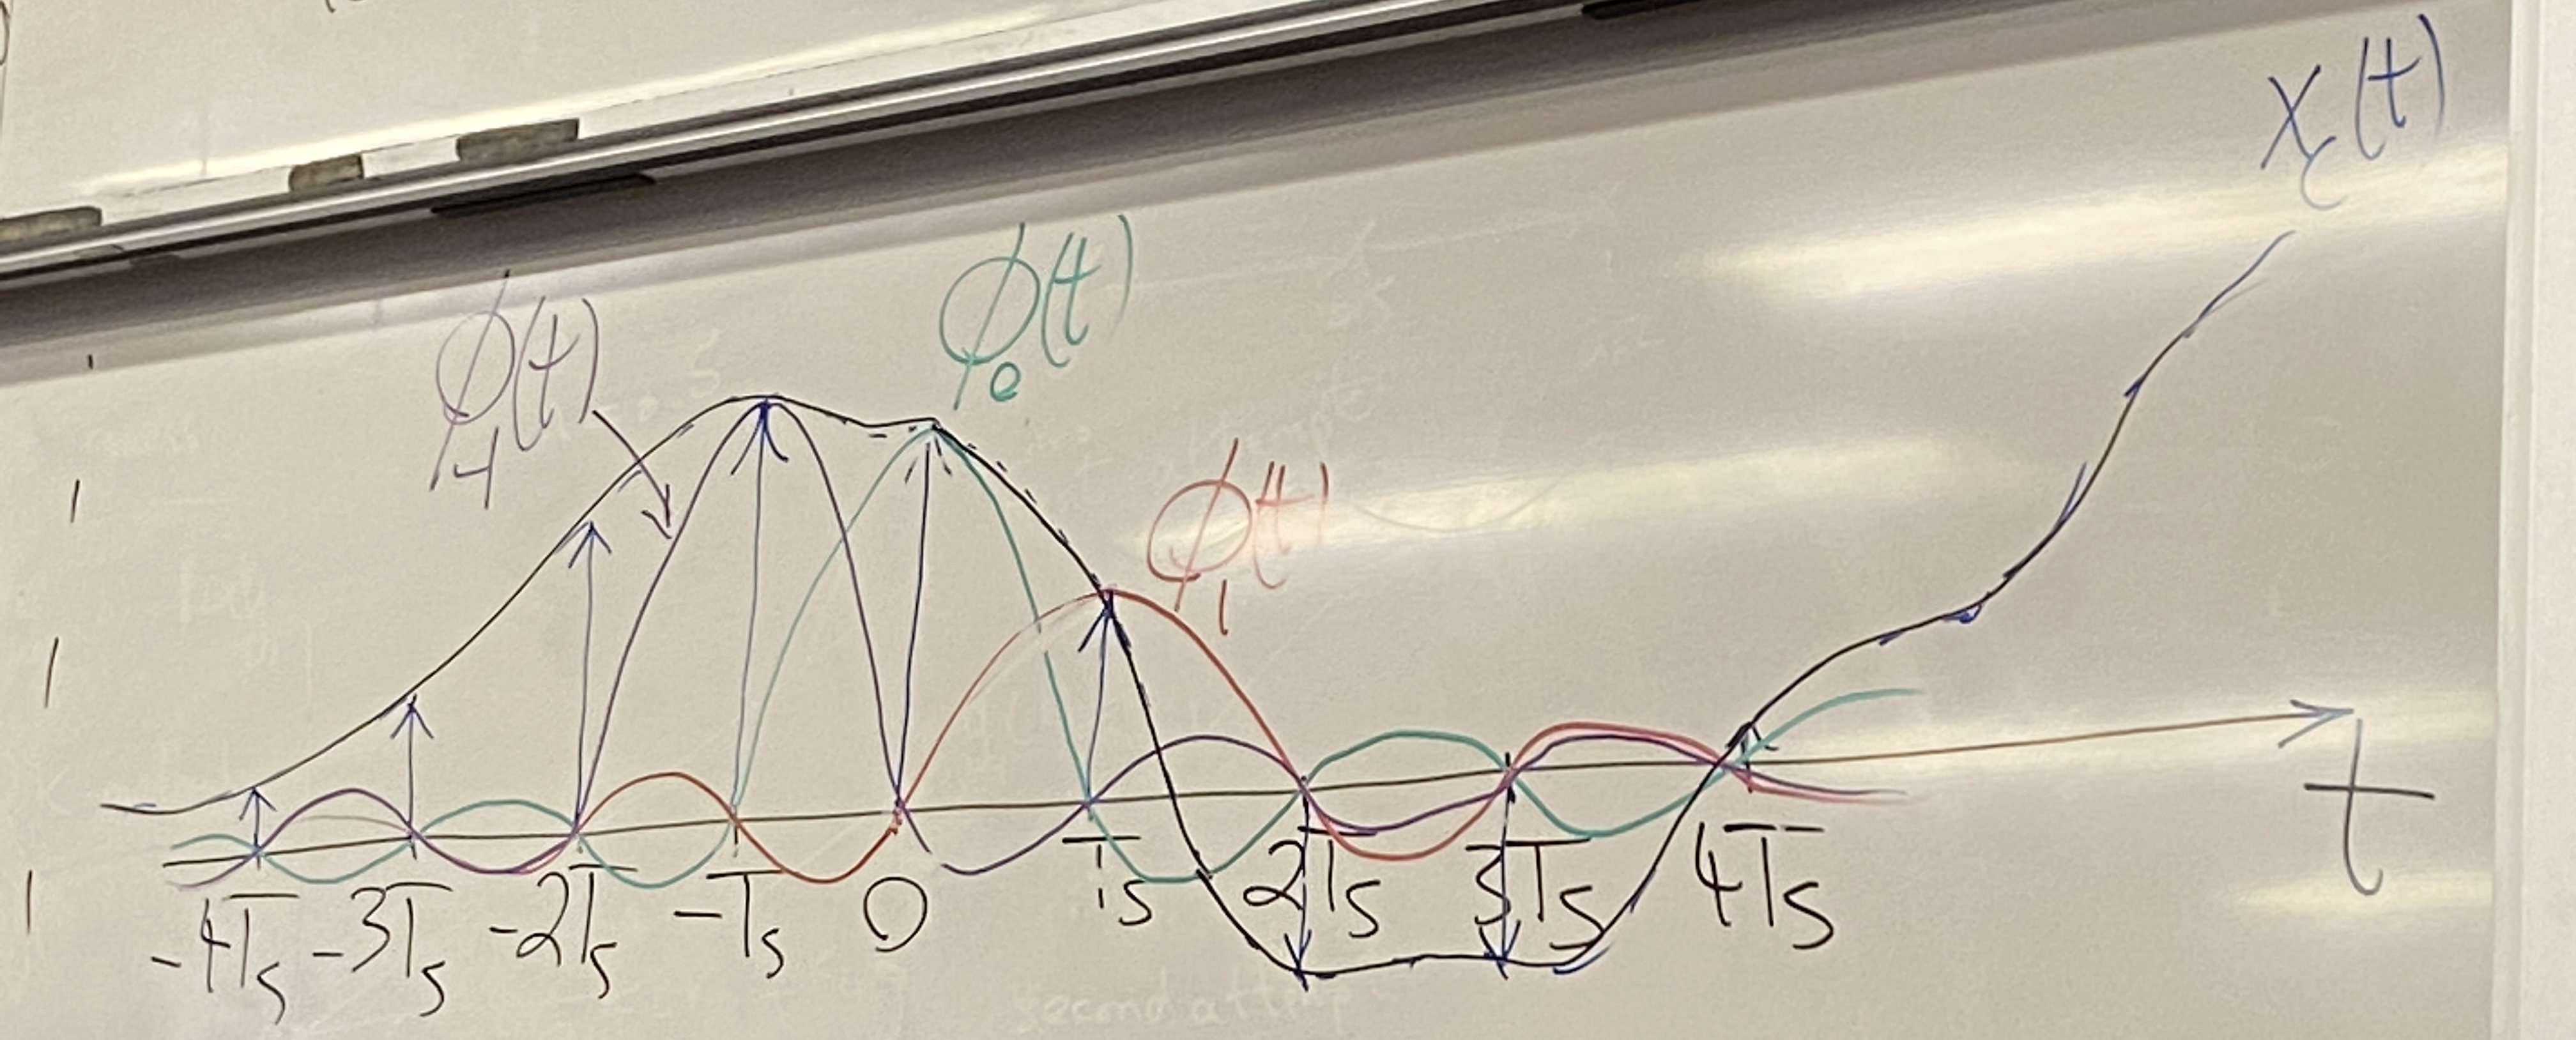
\includegraphics[scale=0.115]{lectures/wk11/img/sinc.jpg}
\end{center}

If $x\in$ space of signals bandlimited to $\frac{\omega_s}{2}$ then the $x_c(t) = \displaystyle\sum_{-\infty}^\infty x_c(\ell T_s)\phi_\ell(t)$.

$\{\phi_\ell(t)\}_{\ell=-\infty^\infty}$ form an orthogonal basis.

If you have taken EE 126 then you may know that $\langle X, Y\rangle \triangleq \mathbb E[XY]$. You can show this definition satisfies he least squares solution via the projection property.

\hrulefill

\subsection{Sampling Continued}
Note that the block diagram shown at the start of the class was not completed.

We know (from before):
\begin{align*}
    x_z(t) 
    &= x_c(t) \sum_{\ell=-\infty}^\infty \delta(t-\ell T_s)
\end{align*}
\begin{shaded}
But what is the transform?
\end{shaded}
\begin{align*}
    X_z(\omega) 
    &= \sum_{\ell} x_c(\ell T_s) \delta(t-\ell T_s)
    \\
    &=\sum_{\ell=-\infty}^\infty x_c(\ell T_s) \delta(t-\ell T_s)
    \\
    &=\sum_{\ell=-\infty}^\infty x_c(\ell T_s) \mathcal F\{\delta(t-\ell T_s)\}
    &&\left[\delta(t)\stackrel{\mathcal F}{\leftrightarrow}1\right]
    \\
    &=\sum_{\ell=-\infty}^\infty x_c(\ell T_s) e^{-i(\omega T_s)\ell}
    &&\left[\delta(t-\ell T_s)\stackrel{\mathcal F}{\leftrightarrow}e^{-i\omega\ell T_s}]\right]
    \\
    &=\sum_{\ell=-\infty}^\infty x_d(\ell) e^{-i(\omega T_s)\ell}
    \\
    &=
    X_d(\Omega)\Big|_{|\Omega = \omega T_s}
    &&\left[X_z(\omega)=X_d(\Omega)\Big|_{\Omega=\omega T_s}\right]
\end{align*}

We can note that the units work out:
\[
    \underbrace{\Omega}_{\text{rad/sample}} = \underbrace{\omega}_{\text{rad/sec}}
    \underbrace{T_s}_{\text{sec/sample}}
\]

\hrulefill
\subsection{Triangle Wave}

We can now look at a Triangle wave with period $2B$, centered at $0$.

Now we expand our horizon to the spectrum of $X_d(\Omega)$. Recall that $\Omega=\omega T_s$.

\begin{align*}
    X_z(\omega)
    &=
    X_d(\Omega)\Big|_{\Omega=\omega T_s}
    \\
    X_d(\Omega)
    &=
    X_z(\omega)\Big|_{\omega=\frac\Omega{T_s}}
    \\
    &=
    \frac1{T_s} X_c(\omega) \Big|_{\omega=\frac\Omega{T_s}},\quad|\Omega|\leq\pi.
\end{align*}

\begin{align*}
    Y_d(\Omega)
    &=
    Y_d(\Omega) H_d(\Omega)\quad |\Omega|\leq \pi
    \\
    &=
    \frac1{T_s} X_c(\omega) \Big|_{\omega=\frac\Omega{T_s}}H_d(\Omega)
\end{align*}

\hrulefill

Now we can send $y_d(n)$ and $T_r$ through a Kroneckor-to-Dirac block to get $y_z(t)=\displaystyle\sum_{\ell=-\infty}^\infty y_d(\ell)\delta(t-\ell T_r)$. 

Now we go from Lollipops to Diracs (the inverse of before). \textbf{Note that this step cannot possibly lead to any information loss.}

If we take the Fourier Transform of $y_z(t)$, we get $Y_z(\omega)$.

\begin{align*}
    Y_z(\omega)
    &=\sum_{\ell=-\infty}^\infty y_d(\ell) \mathcal F\{\delta(t-\ell T_r)\} \\
    &= \sum_{\ell=-\infty}^\infty y_d(\ell) e^{-i\omega\ell T_r} \\
    &= \sum_{\ell=-\infty}^\infty y_d(\ell) e^{-i(\omega T_r)\ell} \\
    &\therefore\quad Y_z(\omega)=Y_d(\Omega)\Big|_{\Omega=\omega T_r}
\end{align*}

which gives us the analysis equation for a DT signal!

Passing $y_z(t)$ through a low-pass filter yields $y_c(t)$.

\begin{align*}
    Y_c(\omega) 
    &= G Y_d(\Omega)\Big|_{\Omega=\omega T_r}
    &&\text{[Note the gain interpolates]}
    \\
    &= \frac G{T_s} X_c{\omega}\Big|_{\omega=\frac\Omega{T_s}=\frac{\omega T_r}{T_s}}
    H_d(\Omega)\Big|_{\Omega=\omega T_r}
    \\
    \therefore
    Y_c(\omega) 
    &= \frac G{T_s}X_c\left(\frac{\omega T_r}{T_s}\right) H\left({\omega T_r}\right)
\end{align*}

\hrulefill

\subsection{Overall System}

Overall, the final end-to-end system is the input $x_c(t)$ sent through a $C$-to-$D$ block with $T_s$ to get $x_d(n)$.

We then pass that into a $H_d(\Omega)$ to get $y_d(n)$ which we then pass through a $D$-to-$C$s block (with $T_r$) to get $y_c(t)$.

% Per req of Pei

\hrulefill

\subsection{LTI Equivalent Systems}
Note that although \textbf{sampling is not an LTI operation} (shifting the input will not lead to shifted sampled); however there is an LTI equivalent which has the frequency response $H_c(\omega)$.
\begin{align*}
    T_s = 
    &T_r = T
    \\
    Y_c(\omega) 
    &= \frac{G}{T} X_c(\omega) H_d(\omega T) 
    \\
    Y_c(\omega) 
    &= \frac{G}{T} H_d(\omega T) X_c(\omega)
\end{align*}

\subsection{Something fun to do}

\begin{align*}
    H_d(\Omega)
    &=1
    \\
    G
    &= 2T_s
    \\
    T_r
    &= 2T_s
    \\
    Y_c(\omega) 
    &= ?
    &&\text{[Want to find]}
    \\
    Y_c(\omega) 
    &=
    \frac G{T_s}X_c\left(\frac{\omega T_r}{T_s}\right) H\left({\omega T_r}\right)
    &&\text{[Eqn. from before]}
    \\
    Y_c(\omega) 
    &=
    2X_c(2\omega)
    \\
    \implies
    y_c(t) 
    &= 
    x_c(\frac t2)
\end{align*}
Here we compress in frequency which dilates in time.

This means that voice is at half the speed, half the pitch.
